\documentclass[journal]{IEEEtran}

\ifCLASSINFOpdf
\else
\fi

\usepackage{amssymb}
\usepackage{amsthm}
\usepackage{indentfirst}
\usepackage{graphicx}
\usepackage{caption}
\usepackage{algorithm}
\usepackage{algorithmicx}
\usepackage{algpseudocode}
\usepackage{tabularx}
\usepackage{multirow}
\newcommand{\tabincell}[2]{\begin{tabular}{@{}#1@{}}#2\end{tabular}}
\usepackage{array}
\usepackage{booktabs}
\usepackage{multirow}

% correct bad hyphenation here
\hyphenation{op-tical net-works semi-conduc-tor}


\begin{document}

\title{Blind Motion Deblurring with Unpaired Dataset using Cycle-Consistent Adversarial Networks}

\author{
Hao~Wang, 515021910060 \qquad Zhiwen~Qiang, 515030910367
}

\maketitle

% As a general rule, do not put math, special symbols or citations
% in the abstract or keywords.
\begin{abstract}
In this project, we study the problem of blind motion deblurring using conditional generative adversial networks. And DeblurGAN\cite{deblurgan} is introduced to solve this problem. DeblurGAN is an end-to-end learning approach with multi-component loss function and it can achieve image deblurring in a very efficient and fast manner. Furthermore, in order to overcome the drawback that DeblurGAN requires pairwise images as the training dataset, we try to implement an unpaired image-to-image translation based on CycleGAN\cite{cyclegan}  to do the blind motion deblurring. And in the evaluation part, we use Mean Squared Error (MSE) and Structural Similarity Index\cite{ssim} (SSIM) to compare the deblurring images. The outcome shows that in most of cases, CycleGAN can achieve better visual result compared with DeblurGAN. And CycleGAN outperforms DeblurGAN in both measure methods.\footnote{Our source code, dataset and other submission materials are avaliable on github: https://github.com/QLightman/VRAR-Course-Project.}
\end{abstract}
% Note that keywords are not normally used for peerreview papers.
\begin{IEEEkeywords}
Image deblurring, Adversarial networks, DeblurGAN, cycleGAN.
\end{IEEEkeywords}

\IEEEpeerreviewmaketitle

\section{Introduction}
\IEEEPARstart{D}{eblurring} is the process of removing blurring artifacts from images, such as blur caused by defocus aberration or motion blur. There are mainly two types of deblurring methods: blind and non-blind deblurring. Many works have been focused on non-blind deblurring in recent years, making an assumption that the blur function is known. Like blur caused by camera shake, etc.

But in many cases, it is not always easy to learn about the blur kernel (the blur function) for deblurring. Thus, in this project, we try to recover the sharp image given only a blurred image as input, so no information about the blur kernel is required. To do that, we train a generator with the help of adversarial networks. For each blurred image, the generator estimates corresponding sharp image.

The overall goal of this project is to achieve image deblurring without knowing about the blur kernel. And to be specific, we use $DeblurGAN$\cite{deblurgan} to deblur images, which is proposed in the original research paper. $DeblurGAN$ is an end-to-end learning approach with multi-component loss function.  In addition, during the training phase, critic function with gradient penalty and perceptual loss is introduced and the networks are trained in an adversarial manner. With pairwise images as its training dataset, image deblurring can be achieved in a very efficient manner. And the speed is five times faster than previous work. Thus considering the features of $DeblurGAN$, it can be applied to large scale image deblurring, e.g. video deblurring etc.

However, the proposed method has some disadvantages. One is that pairwise images are required to train the adversarial networks, which in other words, we need a blurred image as well as its sharp version.  Despite the fact that in the original research paper, the pairwise sharp (real images, from GO Pro camera) and blurred (fake images, generated by blurring algorithm) images are provided, there is no doubt that it is nearly impossible to get the real blurred image and its real sharp version (instead of the synthetic one) at the same time.

Thus, combining with our work last semester, we take advantage of $CycleGAN$\cite{cyclegan} to try to overcome the dataset problem mentioned above and re-implement image deblurring based on it. $CycleGAN$ is used in image style translation. For example, it can translate a horse to zebra or translate a  Monet's painting to a photo-like image (see \textbf{Fig.\ref{sample1}} and  \textbf{Fig.\ref{sample2}}). And $CycleGAN$ only needs image collections as the dataset to train adversarial networks, and each image collection has some feature in common, e.g.,if we want to get a horse to zebra translation(or zebra to horse), a image collection of zebras and a image collection of horses are needed. And in the two collections they have their own feature. Thus pairwise images are no longer required. Our idea is that if we can treat blur and sharpness as a kind of image style, successful image deblurring may be achieved with unpaired image dataset based on $CycleGAN$. And the outcome indeed proves that $CycleGAN$ can achieve similar result to that of $DeblurGAN$ if we properly select the training dataset.
  
Below are roughly all the goals we try to achieve in our project.
\begin{itemize}
	\item Read and fully understand the paper, acquire the dataset and source code for future use.
	\item  Set up the Keras and TensorFlow working environment.
	\item  Select a small dataset to train a sample generator to test the algorithm and obtain a rough result.
	\item Use a server to train a complete generator to test the performance of proposed method.
	\item Try to use $CycleGAN$ to realize the image deblurring and improve the results of the $CycleGAN$.
	\item Complete the final report for the project.
\end{itemize}
\begin{figure}[htbp]
	\centering
	\footnotesize
	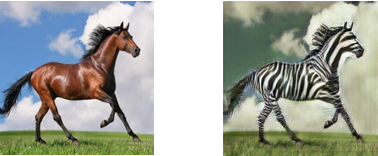
\includegraphics[width=0.8\linewidth]{fig/exam1.jpg}
	\caption{A horse to zebra translation using $CycleGAN$.}
		\label{sample1}
	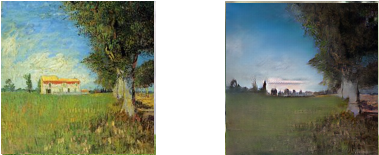
\includegraphics[width=0.8\linewidth]{fig/exam3.jpg}
	\caption{A Monet's painting to photo translation using $CycleGAN$. }
	\label{sample2}
\end{figure}
\subsection{Related Work}
The formulation of blur model can be described as follows:
\begin{equation}
I_B=K*I_S+N
\end{equation}
where $I_B$ is a blurred image, $K$ is a blur kernel, $I_S$ is a sharp image and $N$ is the noise.
 
The deblurring methods can be divided into mainly two types: blind and non-blind deblurring. Early works \cite{early_work} mostly focus on non-blind deblurring, making an assumption that the blur kernel is known. These methods rely on the classical Lucy-Richardson algorithm, Wiener or Tikhonov filter to obtain the estimate $I_S$. 

Since in practice the blur function is unknown, many algorithms rely on image heuristics and assumptions on the source of the blur. Like blur caused by camera shake, etc. Some of the methods are based on an iterative approach \cite{Fergus,Xu}, they use parametric prior model to improve the estimate of the motion kernel and sharp image on each iteration. The shortcoming of these approaches is that the running time is too long and the stopping criterion is hard to control. Others use the local linearity of a blur function and simple heuristics to quickly estimate the unknown kernel. These methods are fast but work well only on a small subset of images.

Over the last few years, with the success of deep learning, there appeared many approaches \cite{Sun} to use CNN to estimate the unknown blur kernel . Chakrabarti \cite{Chakrabarti} uses CNN to predict complex fourier coeffieients  of motion kernel to perform non-blind deblurring in fourier space, Gong \cite{Gong} uses fully convolutional network to move for motion flow estimation. Recently, a kernel-free end-to-end approach \cite{Noroozi,Nah} have been implemented by using multi-scale CNN to directly deblur the image, which can deal with different sources of the blur.

\subsection{Proposed Work in Assigned Research Paper}
The goal is to recover sharp image $I_S$ given only a blurred image $I_B$ as an input, so no information about the blur kernel is provided. To do that we train a CNN $G_{θ_G}$ , to which we refer as the Generator. For each $I_B$ it estimates corresponding $I_S$ image. In addition, during the training phase, we introduce critic function $D_{θ_D}$, and train both networks in an adversarial manner.

\begin{itemize}
	\item Generator\\
	The generator aims at reproducing sharp images. The network is based on ResNet blocks. It keeps track of the evolutions applied to the original blurred image. To be specific, it contains two strided convolution blocks with stride 1/2, nine residual blocks and two transposed convolution blocks. \textbf{Fig.\ref{generator}} depicts the architecture of generator.
	\begin{figure*}
		\centering
		\footnotesize
		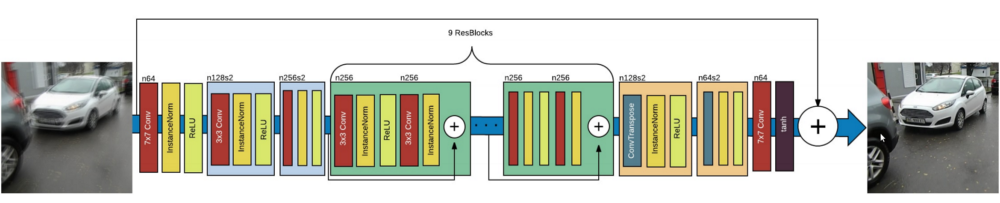
\includegraphics[width=0.8\textwidth]{fig/generator.png}
		\caption{Architecture of the generator. It contains two strided convolution blocks with stride 1/2, nine residual blocks and two transposed convolution blocks.\cite{deblurgan} }
		\label{generator}
	\end{figure*}
	
	\item Loss Function\\
	The loss function consists of adversarial loss and content loss. The full objective is:
	$$
	\mathcal{L}= \mathcal{L}_{GAN} + \lambda\mathcal{L}_{X}
	$$
	where $\lambda$ describes the relative importance of these two losses.\\ 
	For adversarial loss, more recently, \cite{cyclegan} provides an alternative way of using Least Square GAN \cite{Mao} which is more stable and generates higher quality results. The research paper adopts WGAN-GP \cite{Gulrajani} as the critic function. It is calculated as follows:
	$$
	\mathcal{L}_{GAN} = \sum_{n=1}^{N}-D_{\theta_{D}}(G_{\theta_{G}}(I^B))
	$$

	For content loss,the original paper adopts Perceptual loss \cite{Gulrajani}. Perceptual loss is based on the difference of the generated and target image feature maps:
	$$
	\mathcal{L}_{X} = \frac{1}{W_{i,j}H_{i,j}}\sum_{x=1}^{W_{i,j}}\sum_{y=1}^{H_{i,j}}(\Phi_{i,j}(I^S)_{x,y}-\Phi_{i,j}(G_{\theta_G}(I^B))_{x,y})^2
	$$
	where $W_{i,j}$ and $H_{i,j}$ are the dimensions of the feature maps and $\Phi_{i,j}$ is the feature map. 
	
\end{itemize}
\subsection{Limitations of Proposed Work}
The main limitations of the proposed work is that the training process of $DeblurGAN$ require pairwise dataset, as is shown in \textbf{Fig.\ref{keras_dataset}}, which is hard to obtain in real world. Althought $DeblurGAN$ provide a method of generating synthetic motion blurred images from the sharp ones, the performance of using fake 'blurred' images only is unpromising. So lack of training dataset restrains the scope of application of $DeblurGAN$. 
\begin{figure}[htbp]
	\centering
	\footnotesize
	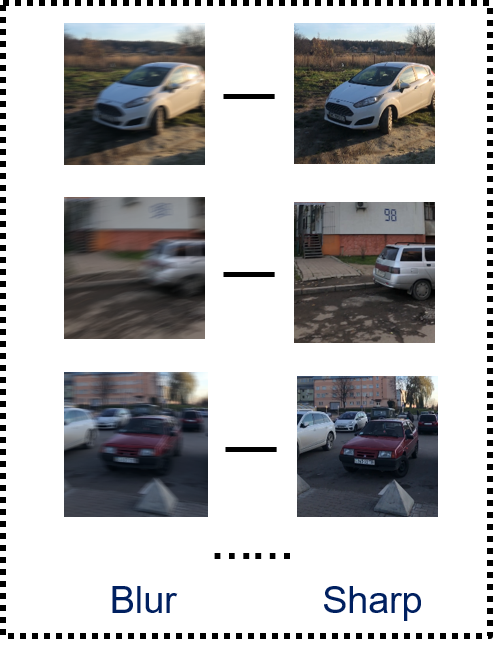
\includegraphics[width=4cm]{fig/keras_dataset.png}
	\caption{The training dataset of $DeblurGAN$. The one on the left is a blur dataset and the one on the right is its corresponding sharp version.}
	\label{keras_dataset}
\end{figure}

\section{Methodology} 
In our work, we firstly implement the $DeblurGAN$ and then use $CycleGAN$ to over come the pairwise dataset problem. Thus this part will give the methodology of $DeblurGAN$ and $CycleGAN$.

\subsection{CycleGAN}
One of the significant advantages for $CycleGAN$ is that it is unpaired image-to-image translation. Thus, pairwise image dataset is no longer required.The flow chart of $CycleGAN$ is illustrated in \textbf{Fig.\ref{pipeline}}.
\begin{figure*}
	\centering
	\footnotesize
	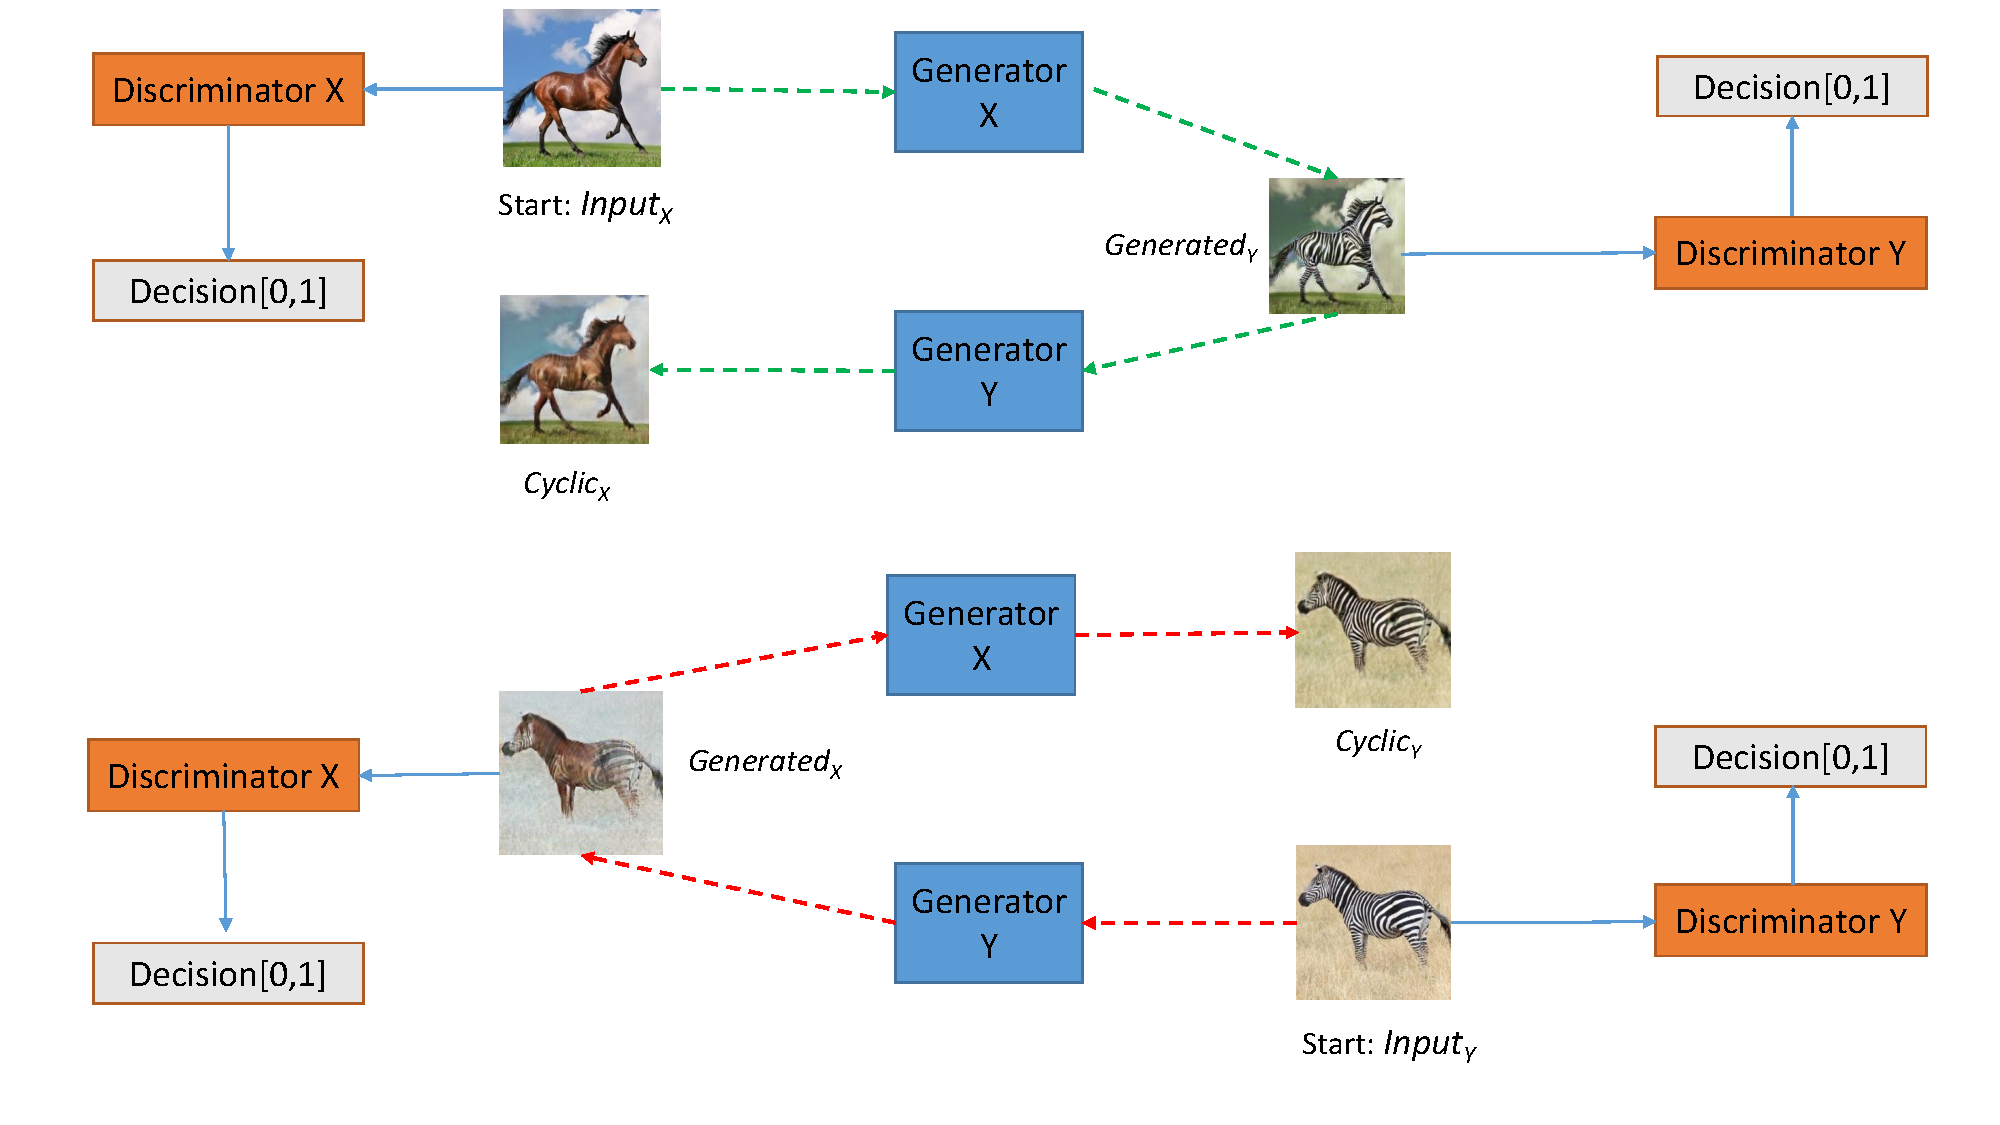
\includegraphics[width=0.8\textwidth]{fig/pipeline.pdf}
	\caption{Architecture of $CycleGAN$.It consists of two generators and two discriminators. The generators' goal is to learn the mapping between two image domains.}
	\label{pipeline}
\end{figure*}
\subsubsection{Generator}
\begin{figure}[htbp]
	\centering
	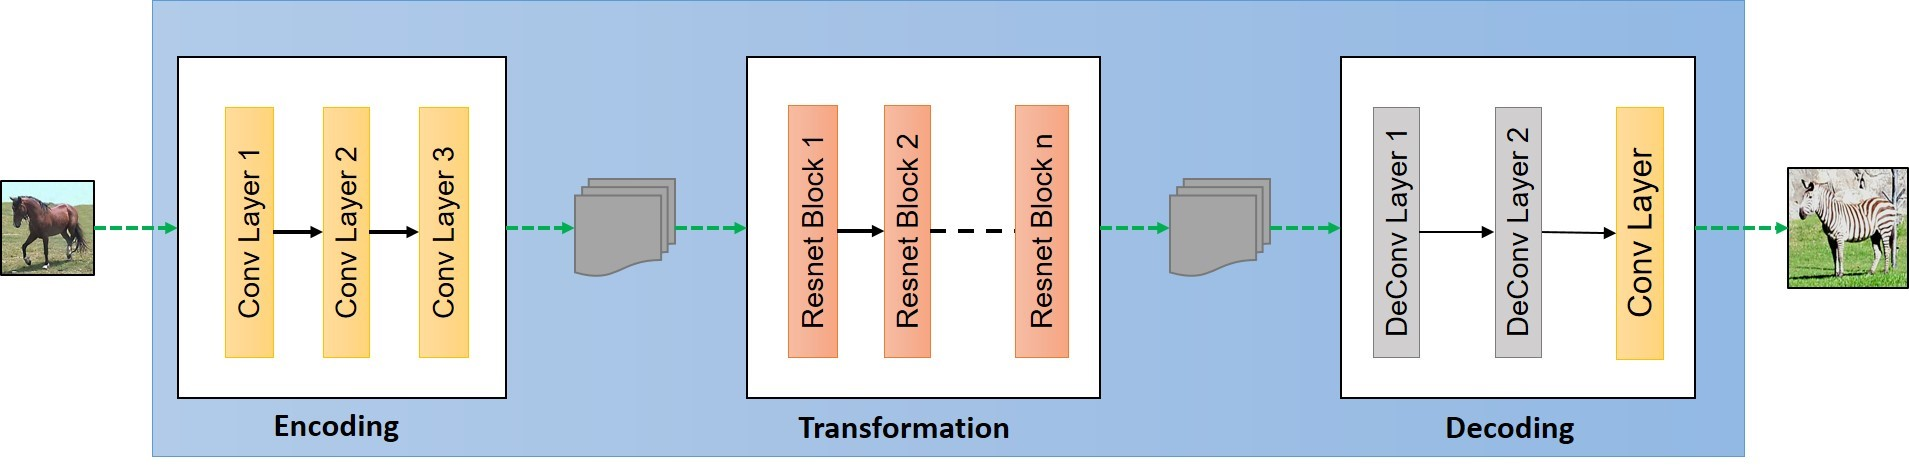
\includegraphics[width=8.5cm]{fig/generator.jpg}
	
	\caption{Generator for the $CycleGAN$}
	\label{fig:Generator}  
\end{figure}
Since two generators work in a same way, Only take Generator X as an example.
Generator X(see \textbf{Fig. \ref{fig:Generator}}) consists of 3 parts: encoder, transformer and decoder.

Following are the parameters we have used for the model.
$$
batch\_size = 1 \# batch\_size
$$
$$
pool\_size = 50 \# pool\_size
$$

\textbf{Encoder.}
For simplicity, the input has been fixed as $[256,256,3]$. The first step is extracting features from an image through a convolution network. A convolution network takes an image as input, and then uses filters to move over the image to extract out features by one stride each time. For the first layer, each filter is $7*7$ and the stride is $1*1$. The activation function is relu.  Output’s shape will be $[256,256,64]$ (by padding). Then, the output of the first layer will be passed to the second layer, and so on. 

The hyperparameters of the second layer is:\\
$ \#filters=128, filter= 3*3, stride=2*2,\\
 activation function is relu, \\
 output= [128,128,128].$

The hyperparameters of the third layer is: \\
$\#filters=256, filter= 3*3, stride=2*2, \\
activation function is relu, \\
output= [64,64,256]$.

So, the input of the transformer will be $[64,64,256]$, meaning 256 features vectors of size $64*64$ each.\\

\textbf{Transformer.}
This part is to transform feature vectors of an image from domain $X$ to domain $Y$. To do so, we have used 6 layers of resnet blocks. All filters’ size is $3*3$ and stride is $1*1$. Output is $[64,64,256]$.

\textbf{Decoder.}
Decoding step is exactly opposite of encoding step. We will rebuild an image from those feature vectors gained before, and this is done by applying three deconvolution layers which uses reversed parameters of encoding step.

\subsubsection{Discriminator}
\begin{figure}[htbp]
	\centering
	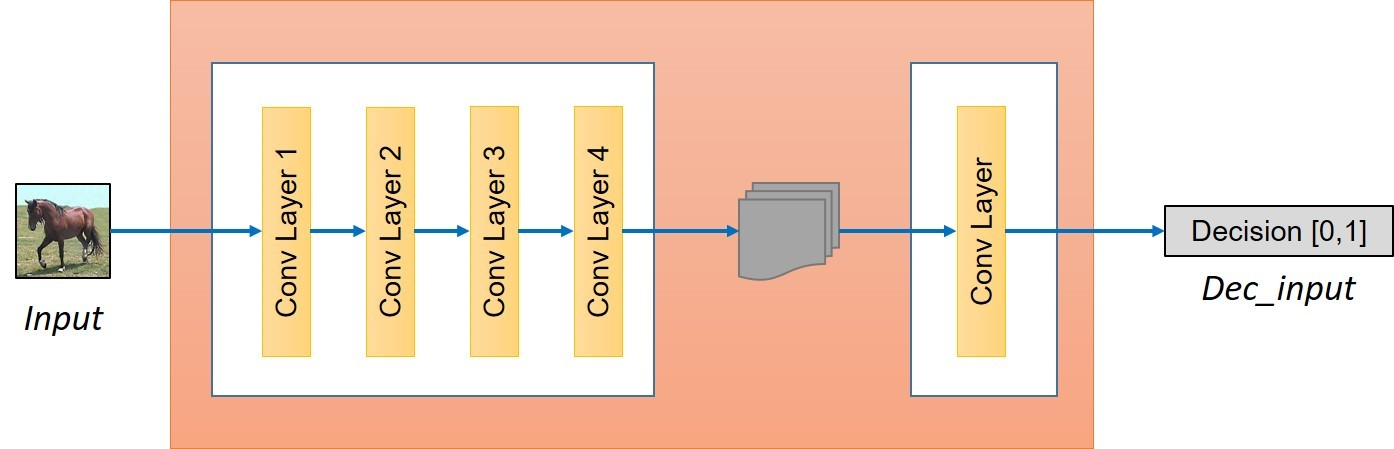
\includegraphics[width=8.5cm]{fig/Discriminator.jpg}
	\caption{Discriminator for the $CycleGAN$}
	\label{fig:Discriminator}
\end{figure}

Discriminator(see \textbf{Fig. \ref{fig:Discriminator}}) also needs to extract features, so it’s basically a convolution network.Next step is deciding whether these features belongs to that particular category or not. For that we add a final convolution layer which produces a 1-dimensional output.

Hyperparameters: $$\#filters + filter size + stride + activation function$$
$$Layer1: 64, 4*4, 2, leakyrelu (slope=0.2)$$
$$Layer2: 128, 4*4, 2, leakyrelu (slope=0.2)$$
$$Layer3: 256, 4*4, 2, leakyrelu (slope=0.2)$$
$$Layer4: 512, 4*4, 2, leakyrelu (slope=0.2)$$
$$decision = 1, 4*4, 1, least square gan$$

All filters are initialized by $tf.random\_normal\_initializer()$ function with $Gaussian's\, mean=0$ \& $standard\, deviation=0.02$

\subsubsection{Loss} 
We use least square $GAN$ loss, to meet our goal, the loss function must satisfy:
Discriminator $X$ must be trained such that recommendation for images from domain $X$ must be as close to 1. So, discriminator $X$ would like to minimize $(Discriminator X(x)-1)^2$.\\
Also, since discriminator $X$ should be able to distinguish generated and original images, it should predict 0 for images produced by the generator $X$. Discriminator $X$ would like to minimize $(Discriminator X (Generator Y\rightarrow X(y)))^2$.\\
Moreover, generator $X$ should eventually be able to fool the discriminator $Y$ about the authenticity of its generated images. This can be done if the recommendation by discriminator $Y$ for the generated images is as close to 1 as possible. So, generator $X$ would like to minimize $(Discriminator Y (Generator X\rightarrow Y(x))-1)^2$.

And the most important cycle loss captures that we are able to get the image back using another generator and thus the difference between the original image and the cyclic image which is $[F (G(x))-x] + [G(F(y))-y]$ should be as small as possible.

PS: weights of both cycle losses are 10 compared with other losses.


\subsection{DeblurGAN}
This adversarial networks consists of generator and discriminator. And some of its structures are similar to that in $CycleGAN$. Thus here is a simple explaination for $DeblurGAN$. Following are the parameters we have used for training the model.\\
$
batch\_size = 16,\\
epoch\_num = 50,\\
num\_discri\_training = 5.
$
\subsubsection{Generator}
The generator aims at reproducing sharp images. It is based on ResNet blocks. And the nine ResNet blocks applied to an unsampling of the original image. This ResNet layer is basically a convolutional layer, with input and output added to form the final output.\\
Resnet block can be summarized as follows, which contains a direct channel from the input to the output and two convolution layers.
\begin{figure}[htbp]
	\centering
	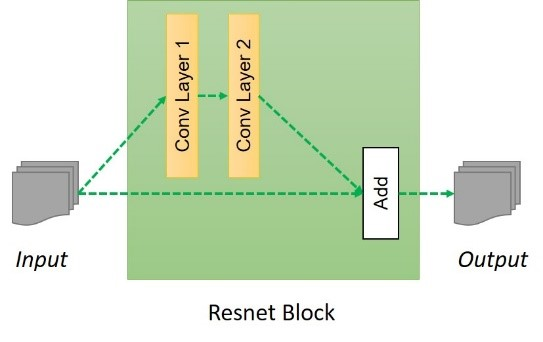
\includegraphics[width=8.5cm]{fig/resnet.jpg}
	\caption{Resnet for the $DeblurGAN$}
	\label{fig:resnet}
\end{figure}
The reason for using Resnet block(see \textbf{Fig.\ref{fig:resnet}}) is to ensure properties of input of previous layers are available for later layers, so that the output do not deviate much from original input, otherwise the characteristics of original images will not be retained in the output like the size and shape of the object and results can be very abrupt.
The hyperparameters of nine ResNet blocks are: \\
$
ngf = 64,\\
input\_nc = 3,\\
output\_nc = 3,\\
input\_shape\_generator = (256, 256, input\_nc),\\
n\_blocks\_gen = 9
$ 

\subsubsection{Discriminator}
The objective of discriminator is to determine if an input image is artificially created. Therefore, the discriminator’s architecture is convolutional and outputs a single value.\\
The hyperparameters of nine ResNet blocks are: \\
$
ndf = 64,\\
output_nc = 3,\\
input_shape_discriminator = (256, 256, output_nc)
$
\section{Implementation}
\begin{itemize}
\item We have implemented our $DeblurGAN$ with the Keras framework. We successfully constructed the generator and discriminator according to the methodology part. Then we trained our model on a random crops of size 256x256 from the light version (9GB) of the GOPRO dataset, which contains artificially blurred images from multiple street views. The training time was around 1 hour (for 50 epochs) on two Titan Xp GPUs.
\item We have implemented our $CycleGAN$ on motion deblurring with the help of Googles TensorFlow framework. We have successfully constructed the $CycleGAN$ by using several TensorFlows API which are implemented in Python, the unpaired dataset we use consists of 561 sharp images and 560 blurred images of size 256*256. Besides, we have also tried to use the GOPRO dataset to train $CycleGAN$.
\end{itemize}

\section{Results}
\subsection{Results of DeblurGAN}
We have successfully achieved $DeblurGAN$. And using corresponding method mentioned above to re-implement it.
\textbf{Fig.\ref{fig:result}}  are part of what we have achieved. And in the deblurred images, the edges of most objects are much clearer.  So as we can see, this adversarial network can achieve good results as we have expected.
\begin{figure*}
	\centering
	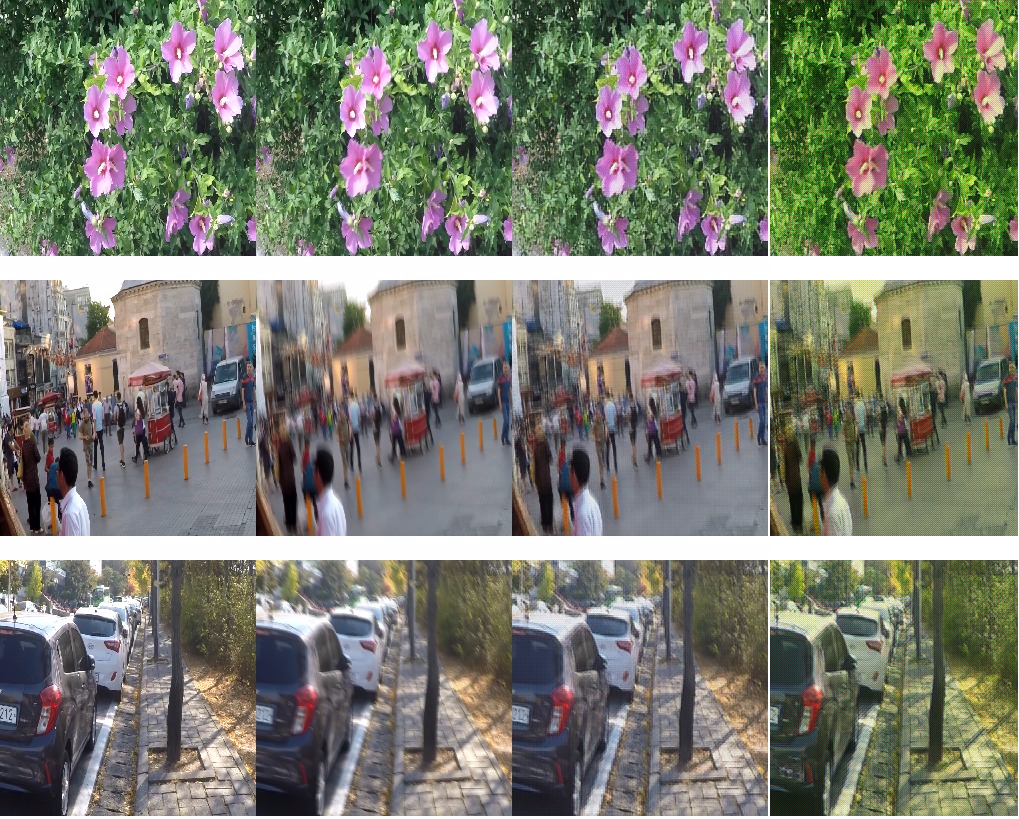
\includegraphics[width=0.8\textwidth]{fig/result.png}
	\caption{ Images processed by $DeblurGAN$. From left to right: ground truth sharp image, blurred photo, result of $DeblurGAN$ obtained by us, result of $DeblurGAN$ presented in the paper \cite{deblurgan}. }
	\label{fig:result}
\end{figure*}
\subsection{Results of CycleGAN}
We have also successfully achieved $CycleGAN$. And using corresponding method mentioned above to re-implement it. Since $CycleGAN$ has the property of cycle-consistency, which means we can deblur images and blur sharp images as well. As is shown in \textbf{Fig.\ref{fig:cycle}}. If we transform from source distribution to target and then back again to source distribution, we should get samples very similar to our source distribution. 
\begin{figure}[htbp]
	\centering
	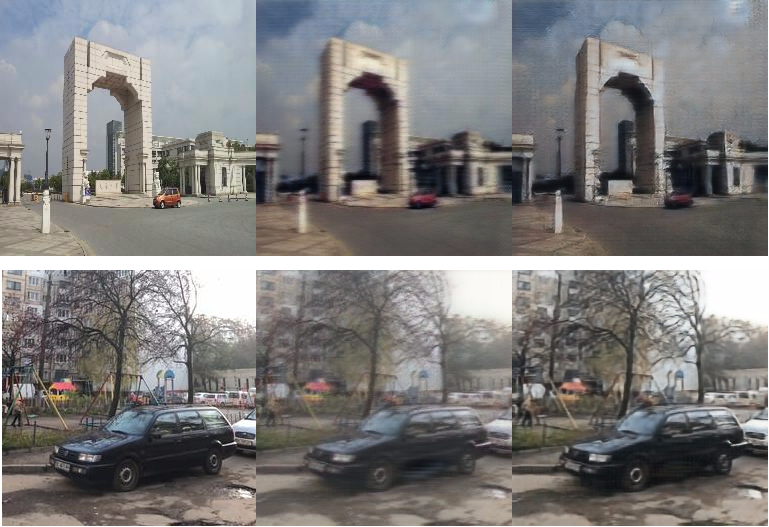
\includegraphics[width=8.5cm]{fig/cycle.png}
	\caption{ Images processed by $CycleGAN$. From left to right: A(ground truth sharp image), B(A blurred by $CycleGAN$), C(B deblurred by $CycleGAN$).}
	\label{fig:cycle}
\end{figure}

\textbf{Fig.\ref{fig:cyclegan}} shows the results of deblurring images using $CycleGAN$, it is worthy noting that since we use unpaired images as training dataset, we do not have the ground truth sharp image, but based on our prior knowledge, it is true that successful image deblurring can be achieved with unpaired image dataset using $CycleGAN$. Moreover, the idea of treating blur and sharpness as a kind of image style actually works. Also, a by-product of generating fake blurring images using CycleGAN are also provided.

\begin{figure}[htbp]
	\centering
	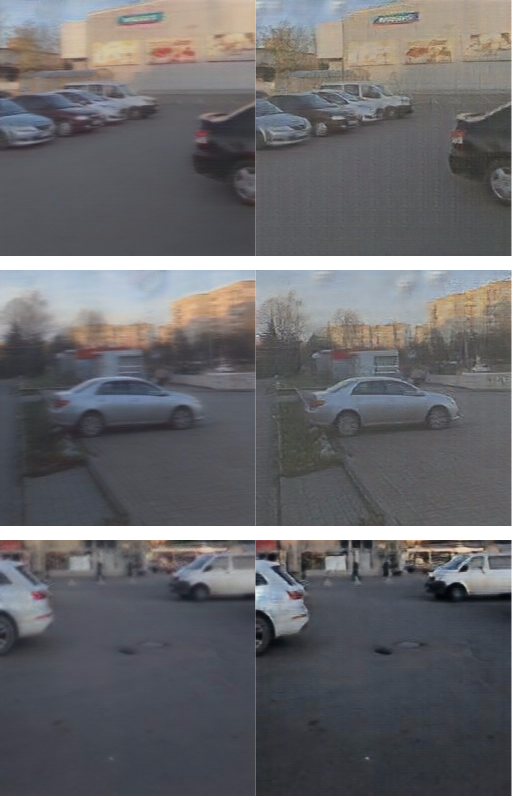
\includegraphics[width=8.5cm]{fig/cyclegan.png}
	\caption{ Images processed by $CycleGAN$. From left to right: blurred photo, result of $CycleGAN$.}
	\label{fig:cyclegan}
\end{figure}
\subsection{Metrics of Comparison}
In order to compare the deblurring results, we try to calculate the image similarity between the original sharp image and the deblurred one (deblurred by two $GAN$ networks correspondingly). It is very intuitive that the higher the similarity is, the better deblurring result we achieve.

And two metrics are introduced to measure the similarity. One is Mean Squre Error (MSE) and the other is Structural Similarity Index\cite{ssim} (SSIM). And in this problem the second is more rational as is explained below.
\subsubsection{Mean Squre Error}
The equation for MSE is:
$$E = \frac{1}{mn} \sum_{i=0}^{m-1}\sum_{j=0}^{n-1}[I_{ori}(i,j) - I_{deblur}(i,j)]^2$$
where $E$ is the Mean square error, $I_{ori}$ is the original image, $I_{deblur}$ is the deblurred image and $m,n$ is the size of the image.  

It is important to note that a value of 0 for MSE indicates perfect similarity and the similarity decreases as the value increases.

When using it for similarity, one problem is that large distances between pixel intensities do not necessarily mean the contents of the images are dramatically different, e.g. one image and its low brightness version, they are very similar but with very large mean square error.
\subsubsection{Structural Similarity Index}
The equation for SSIM is:
$$ I(x,y) = \frac{(2\mu_x\mu_y +c_1)(2\sigma_{xy}+c_2)}{(\mu_x^2+\mu_y^2+c_1)(\sigma_x^2+\sigma_y^2+c_2)}$$

where $I$ is the Structutal Similarity Index, $(x,y)$ is a coordinate indicating a nearby $N*N$ window, $\sigma_x$, $\sigma_y$, is the variance of intensities in $x,y$ direction,  $\sigma_{xy}$ is the covariance and $\mu_x$, $\mu_y$ is the average intensity in $x,y$ direction.

Unlike MSE, the SSIM value can vary between -1 and 1, where 1 indicates perfect similarity.

It is worth to note that the SSIM takes the nearby pixels of the pixel at $(x,y)$ into consideration instead of exact pixel to pixel comparison.

\subsection{Result of Comparison}
In this part, we compare the results of image deblurring with $DeblurGAN$ and $CycleGAN$. Part of the results are shown in \textbf{Fig.\ref{fig:compare}}. 

\begin{figure}[htbp]
	\centering
	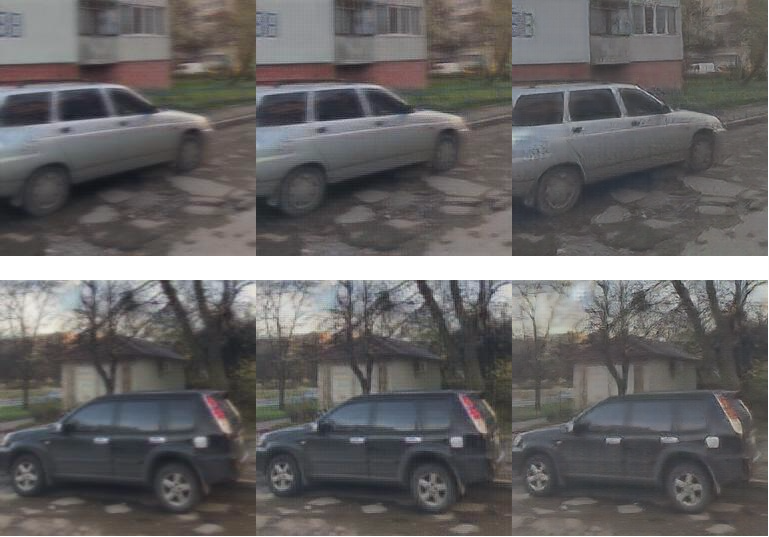
\includegraphics[width=8.5cm]{fig/compare.png}
	\caption{Results of image deblurring with $DeblurGAN$ and $CycleGAN$. From left to right: blurred photo, result of $DeblurGAN$, result of $CycleGAN$.}
	\label{fig:compare}
\end{figure}

Based on the two metrics above, we compare the results by $DeblurGAN$ and $CycleGAN$ using a test dataset of 216 images. Here we calculate the similarity of original sharp image and the deblurred one using either $DeblurGAN$ or $CycleGAN$. 

The result is shown in \textbf{Tab.\ref{com_res}}, \textbf{Fig.\ref{res_ssim}} and \textbf{Fig.\ref{res_mse}}. And to be specific, according to SSIM, about $69\%$ out of all test images using $CycleGAN$ outperforms that using $DeblurGAN$. And from the table, in a general sense, the result of $CycleGAN$ is better than that of $DeblurGAN$ because of a higher SSIM and lower MSE. Thus we can draw the conclusion that $CycleGAN$ can achieve better visual result compared with $DeblurGAN$. And in most of the cases, $CycleGAN$ outperforms $DeblurGAN$ in image deblurring.

\begin{table}  
	\caption{CycleGAN and DeblurGAN comparison}
	\label{com_res}  
	\begin{center}  
		\begin{tabular}{l|l|l}  
			\hline  
			Metric & $DeblurGAN$ & $CycleGAN$(ours)   \\
			\hline
			SSIM & 0.737  & 0.784 \\
			MSE & 667.3 & 565.7 \\
			\hline  
		\end{tabular}  
	\end{center}  
\end{table}  

\begin{figure}[htbp]
	\centering
	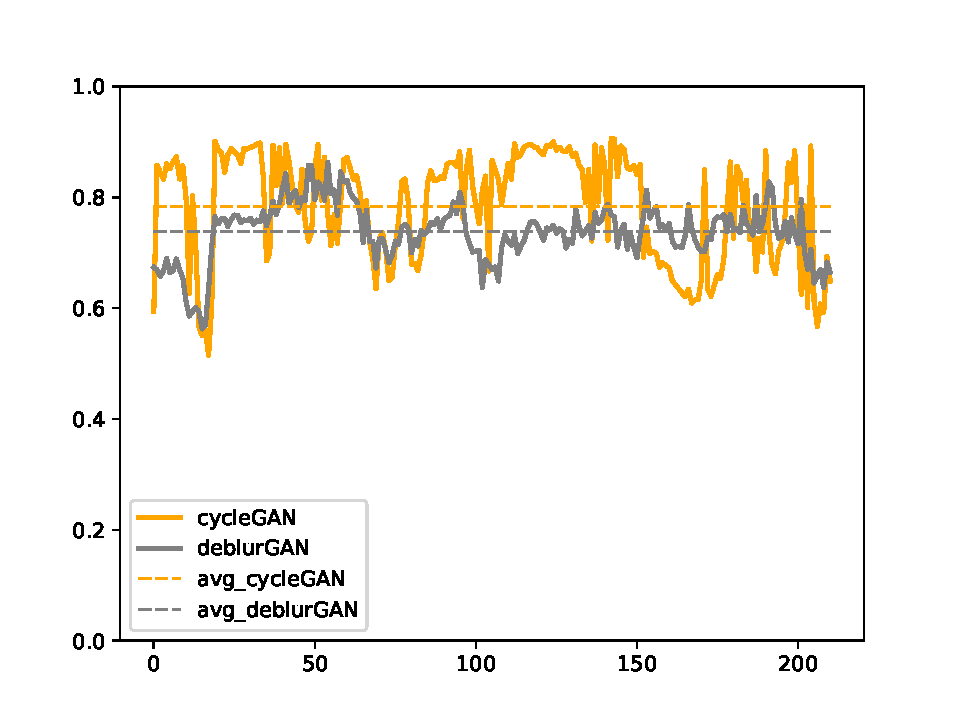
\includegraphics[width=8cm]{fig/Figure_ssim.pdf}
	\caption{Result with SSIM measurement.}
	\label{res_ssim}
\end{figure}
\begin{figure}[htbp]
	\centering
	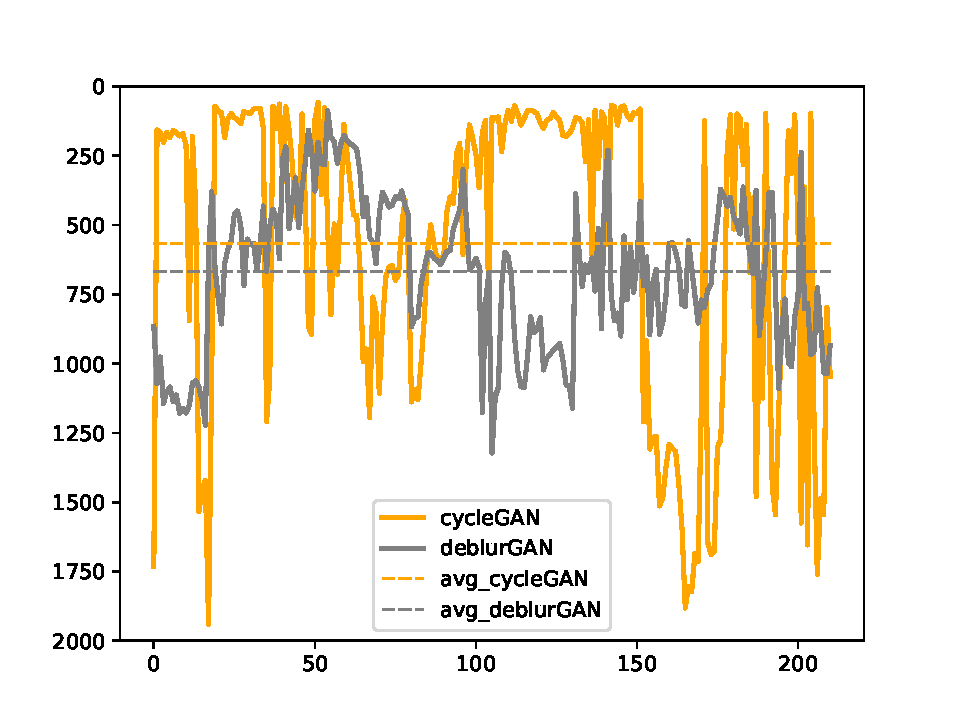
\includegraphics[width=8cm]{fig/Figure_mse.pdf}
	\caption{Result with MSE measurement.}
	\label{res_mse}
\end{figure}
\section{Conclusion and Future Direction}
In this paper, we study the problem of Blind Motion Deblurring. First we use $DeblurGAN$ which is presented in the original paper to reimplement it. Futhermore, as the training of $DeblurGAN$ requires pairwise dataset, while $CycleGAN$, our last semester's project, can perform image to image translation with unpaired dataset, we then focus on applying blind motion deblurring with unpaired dataset using $CycleGAN$. We want to prove that the idea of treating blur and sharp as a kind of image style is practical and $CycleGAN$ can be used to deblur images. And the results show  $CycleGAN$ can achieve similar result to that of $DeblurGAN$.

Since $CycleGAN$ can do all kinds of style translation, and it is not easy for the GAN networks to capture a specific kind of feature if too many noises are in image collections. So if we construct the dataset unproperly, the deblurring process is very likely to fail, as is shown in \textbf{Fig.\ref{fig:bad}}.  The output image changes the color of original image, from red to yellow, which is not expected. So our future work will mainly focus on decreasing the overall sensitivity or increasing one specific style's sensitivity(blur and sharp, ect.) of the $GAN$ network and try to enhance the usability of CycleGAN in image deblurring.
\begin{figure}[htbp]
	\centering
	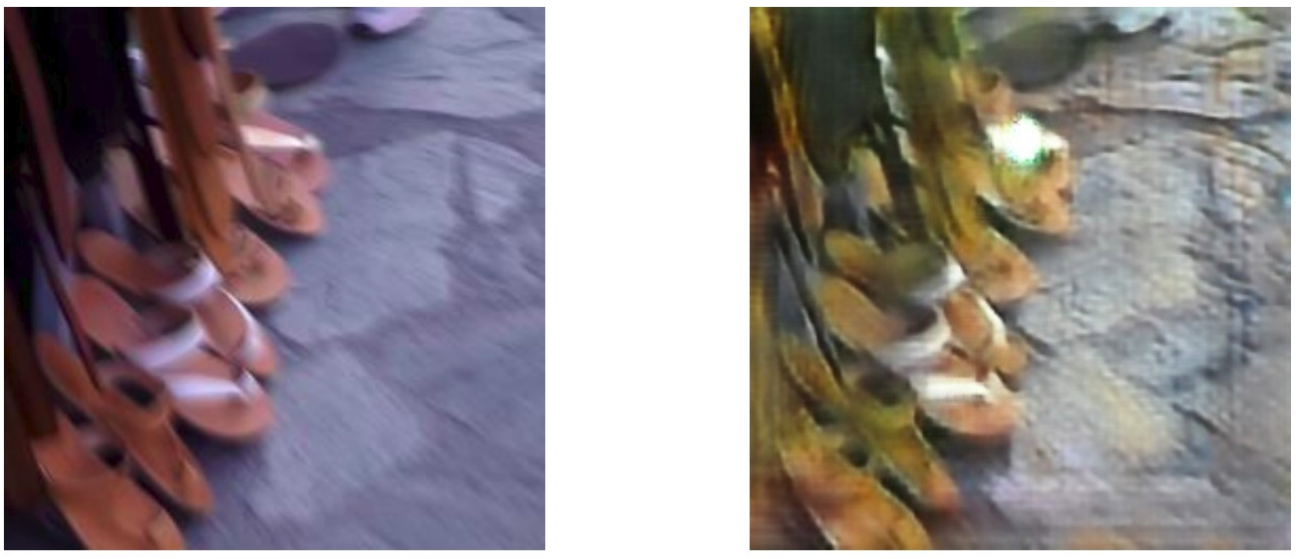
\includegraphics[width=8.5cm]{fig/bad_result.png}
	\caption{ Images processed by $CycleGAN$. From left to right: image blurred photo, result of $CycleGAN$.}
	\label{fig:bad}
\end{figure}


\ifCLASSOPTIONcaptionsoff
  \newpage
\fi

\bibliographystyle{IEEEtran}
\bibliography{ref}

\end{document}


